
%(BEGIN_QUESTION)
% Copyright 2012, Tony R. Kuphaldt, released under the Creative Commons Attribution License (v 1.0)
% This means you may do almost anything with this work of mine, so long as you give me proper credit

This all-pneumatic boiler control system works to regulate the level of water inside the steam drum:

$$\includegraphics[width=15.5cm]{i01152x01.eps}$$

One day the boilerhouse engineer asks you to help him lower the water level inside the steam drum as the boiler is operating.  The water level normally holds at 50\%, but he wants to lower the level to 35\% to perform a test on a low-level water alarm switch recently installed on the drum.  The only problem is, the setpoint on the LIC is non-adjustable, so there is no way to lower the drum level setpoint from 50\% to 35\%.  Neither the LIC nor the FIC has a manual mode.

\vskip 10pt

Devise a way to ``trick'' the control system into lowering the water drum level for an indefinite amount of time needed to perform the engineer's test, given the fact that all these instruments are pneumatic (mechanical), which means their measurement ranges may be adjusted during live operation using nothing but a screwdriver.  Be specific in your description of the solution, and explain why it will work.

\underbar{file i01152}
%(END_QUESTION)





%(BEGIN_ANSWER)

{\it Award half-credit for solutions that would only \underbar{temporarily} lower the steam drum's water level.}

\vskip 10pt

The level transmitter (LT) must be re-calibrated to register {\it 15\% more} level than is actually in the drum, so that the level controller (LIC) works to lower the drum's water level (to get the LT's signal back to 50\% when the real water level is 35\%).

%(END_ANSWER)





%(BEGIN_NOTES)

{\bf This question is intended for exams only and not worksheets!}.

%(END_NOTES)


